\chapter{概述}\label{chapt:intro}

本章涵盖内容包括:

\begin{itemize}
\item Elixir 是什么
\item Elixir 与 Erlang 的不同之处
\item 为什么选择 Elixir 而不是其他语言
\item Elixir/OTP 的适用场景
\item 未来的发展方向
\end{itemize}

如果你是因为药用目的购买了这本书 --- 很抱歉,这是本关于编程语言 Elixir的书。没有其他语言(除了Ruby)让我如此兴奋和乐于使用。即使在花了两年多时间写关于 Elixir的内容之后,我仍然热爱用它编程。

参与一个如此年轻而有活力的社区是一件非常特别的事情。我认为没有哪种语言在v1.0版本之前就已经有至少四本关于它的书、一系列的视频教程和一个会议了。我认为我们正在做一些真正有意义的事情。在深入了解Elixir 之前,我想先谈谈 Erlang 和它传奇的虚拟机,因为 Elixir是建立在它之上的。

Erlang是一种擅长构建软实时、分布式和并发系统的编程语言。它最初的用途是为爱立信的电话交换机编程。电话交换机基本上是连接来电者之间通话的机器。

这些交换机必须是并发的、可靠的和可扩展的。它们必须能够同时处理多个电话。它们还必须极其可靠。没有人希望自己的通话中途被切断。此外,由于软件/硬件故障导致的通话中断不应影响交换机上的其他通话。这些交换机必须能够大规模扩展,并与分布式网络中的其他交换机协同工作。

这些生产需求塑造了今天的Erlang。这些需求正是我们在多核和大规模网络环境中所面临的情况。

正如你将在后面的章节中发现的,Erlang虚拟机的调度器会自动在处理器之间分配工作负载。这意味着,如果你在一个拥有更多处理器的机器上运行程序,你几乎可以\emph{免费}获得速度提升。几乎,因为你需要改变你在Erlang 和 Elixir 中编写程序的思维方式,以获得全部好处。

编写分布式程序,即在不同计算机上运行且能够相互通信的程序,几乎不需要什么仪式性的工作。

现在是时候介绍 Elixir 了。Elixir 自称是\textbf{一个在 Erlang虚拟机之上构建的函数式(Functional)、元编程感知(meta-programming aware)的语言}。让我们逐一解析这个定义。

Elixir是一种\textbf{函数式}编程语言。这意味着它具有你可能期望的所有常见特性,如不可变状态、高阶函数、惰性求值和模式匹配。我们将在后面的章节中遇到所有这些特性以及更多。

Elixir也是一种具有元编程能力的语言。元编程可以描述为生成代码的代码(或者说,黑魔法)。这是可能的,因为代码可以用数据表示,数据也可以用代码表示。这些功能使程序员能够向语言添加新的结构(以及其他事物),而其他语言发现这些功能难以实现,甚至根本不可能实现。

这本书还涉及OTP,一个用于构建容错、可扩展和分布式应用程序的框架。与大多数框架不同,OTP附带了很多优秀的东西。OTP自带三种数据库、一套调试工具、性能分析工具、一个测试框架等等。虽然我们只能玩到一小部分,但这本书将让你体验到OTP 的纯粹精彩。

重要的是要意识到,Elixir本质上是免费获得OTP的,因为 OTP 是 Erlang分发的一部分。如果你想知道OTP是什么意思,简短的答案是它曾经被称为\textbf{开放电信平台(Open Telecom Platform)},这暗示了 Erlang的电信传统。这再次展示了计算机科学中命名是一个难题。这是因为OTP是一个通用框架,与电信几乎没有关系。如今,OTP 就是纯粹的 OTP,就像IBM现在只是 IBM 一样。

\section{Elixir和Erlang有什么不同}

在讨论Elixir与Erlang的不同之处之前,我们先来谈谈他们的\textbf{相似点}。Elixir和Erlang都会编译成相同的字节码。这意味着,无论是Elixir还是Erlang编写的程序,在编译后,都会生成在同一虚拟机上运行的指令。

Elixir的另一个优点是,你可以直接从Elixir调用Erlang代码,反之亦然!例如,如果你发现Elixir缺少Erlang中存在的某些功能,你可以直接从Elixir代码中调用Erlang库函数。

Elixir遵循了Erlang的大多数语义,如消息传递。大多数Erlang程序员会觉得使用Elixir非常自然。

这种互操作性也意味着,丰富的Erlang第三方库资源可以供Elixir开发者(也就是你)使用。那么,为什么你要选择使用Elixir而不是Erlang呢?至少有两个原因 - 工具和生态系统。

\section{工具}

开箱即用的,Elixir自带了一些实用工具:

\subsection{交互式Elixir}

交互式Elixir shell,简称为 \texttt{iex},是一个REPL(读取Read-求值Eval-打印Print 循环Loop),类似于Ruby的\texttt{irb}。它有一些非常棒的功能,如语法高亮和漂亮的文档系统,如图1.1所示。

\begin{figure}[htbp]
  \centering
  % 插入图片文件
  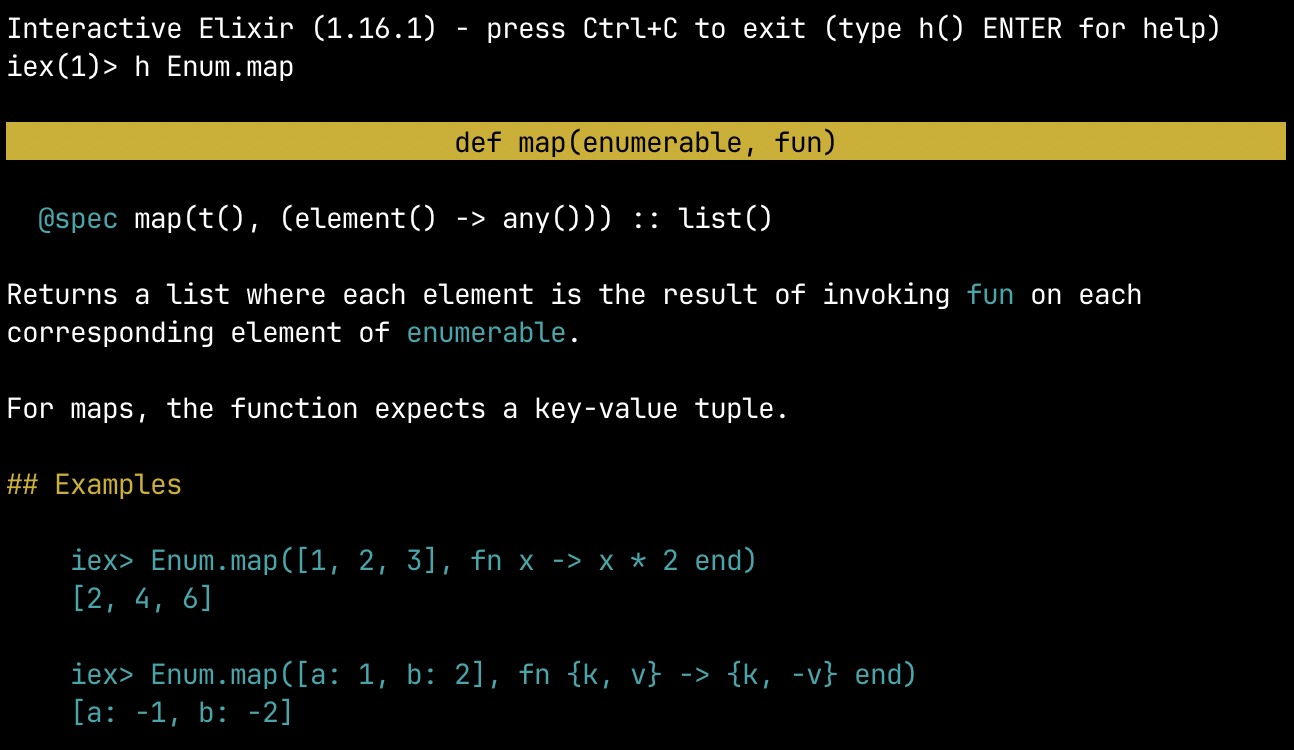
\includegraphics[width=0.8\linewidth]{1_1.png}
  % 添加标题
  \caption{交互式Elixir内置了文档}
  % 添加标签,用于引用
  \label{fig:1_1}
\end{figure}


但\texttt{iex}的功能不止于此!这个工具还允许你连接到\emph{节点},可以理解为可以互相通信的独立Erlang运行时。这些运行时可以存在于同一台计算机、同一局域网或同一网络上。

\texttt{iex}还有一个受Ruby库\texttt{Pry}启发的超能力。如果你之前用过\texttt{Pry},你会知道它是一个允许你深入程序状态的调试器。\texttt{iex}也有一个同名功能,叫做\texttt{IEx.pry}。虽然本书中我们不会使用这个功能,但这是一个非常有价值的工具。以下是如何使用它的简要概述。假设我有这样的代码:

\begin{code}{一个GenServer的示例}
\begin{minted}[linenos]{elixir}
require IEx

defmodule Greeter do
  def ohai(who, adjective) do
    greeting = "Ohai!, #{adjective} #{who}"
    # <--- 这里
    IEx.pry()
  end
end
\end{minted}
\label{lst:genserver_example}
\end{code}

\texttt{IEx.pry}这一行会使解释器暂停,允许我检查传入的变量。首先,我会运行这个函数:

\begin{code}{}\begin{minted}[linenos]{bash}

iex(1)> Greeter.ohai "leader", "glorious"
Request to pry #PID<0.62.0> at ohai.ex:6

    def ohai(who, adjective) do
        greeting = "Ohai!, #{adjective} #{who}"
        IEx.pry
    end
end

Allow? [Yn] Y
\end{minted}
% \caption{Listing Caption}
% \label{lst:id}
\end{code}

一旦我回答 \texttt{Y},我就会进入 \texttt{iex},在那里我可以开始检查传入的变量

\begin{code}{}\begin{minted}[linenos]{bash}
Interactive Elixir (1.2.4) - press Ctrl+C to exit (type h() ENTER for help)
pry(1)> who
"leader"
pry(2)> adjective
"glorious"
\end{minted}
% \caption{Listing Caption}
% \label{lst:id}
\end{code}

在使用\texttt{iex}的过程中,你还会发现其他一些不错的功能,比如\emph{自动补全}。几乎每次Elixir的更新都会给\texttt{iex}带来一些改进和额外的辅助函数,记得跟踪变更日志!

\subsection{使用ExUnit进行测试}

Elixir内置了一个测试框架,名为\texttt{ExUnit}。\texttt{ExUnit}有一些非常好的功能,比如能够\emph{异步}运行,还能产生美观的失败信息,如图1.2所示。ExUnit之所以能够在错误报告方面做出巧妙的处理,主要是因为\emph{宏},我们在本书中不会涉及这个话题。尽管如此,这仍然是一个值得探索的有趣话题。

\begin{figure}[htbp]
  \centering
  % 插入图片文件
  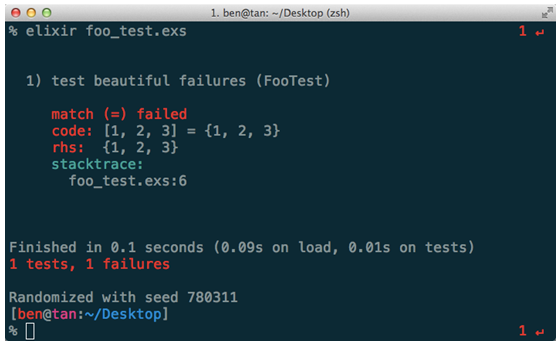
\includegraphics[width=0.8\linewidth]{1_2.png}
  % 添加标题
  \caption{ExUnit 提供了出色的错误信息}
  % 添加标签,用于引用
  \label{fig:1_2}
\end{figure}

\subsection{Mix}\label{mix}

Mix 是一个构建工具,用于创建、编译、测试 Elixir项目。它还用于管理依赖关系等。可以将其类比为 Ruby 中的\texttt{rake} 和 Clojure 中的
\texttt{lein}。事实上,一些最初为\texttt{mix} 做出贡献的开发者也参与了\texttt{lein} 的编写。例如 Phoenix 网络框架就使用 Mix来创建生成器,从而减少编写不必要的样板代码。


\subsection{标准库}

Elixir 自带了一个出色的标准库。数据结构如范围、严格和惰性枚举API,以及合理的字符串操作方式等,都是其中的亮点。

虽然 Elixir可能不是编写脚本的最佳语言,但它包含了一些听起来很熟悉的库,如\texttt{Path} 和\texttt{File}。其文档也非常易用。解释清晰、简洁,并附有如何使用各种库及其函数的示例。

Elixir 拥有一些标准 Erlang 库中没有的模块。我最喜欢的其中之一是\texttt{Stream}。流基本上是可组合的、惰性的枚举。它们通常用于模拟潜在的无限值流。

Elixir 还向 OTP 框架增加了功能。例如,它增加了许多抽象,如\texttt{Agent}来处理状态,\texttt{Task}来处理一次性异步计算。这两者都是基于默认随 OTP 提供的\texttt{GenServer}(代表\emph{通用服务器})构建的。


\subsection{元编程}

Elixir具有类似LISP的宏功能,只是没有括号。宏用于通过用现有构造表达新构造来扩展Elixir语言。语言实现在整个语言中广泛使用宏。库作者也广泛使用它来减少样板代码(Boilerplate code)。

\subsection{生态系统}

作为一种相对较新的编程语言,Elixir建立在一个坚实且经过验证的语言之上,这无疑带来了其优势。


\subsubsection{感谢你,Erlang!}

我认为Elixir最大的收获是来自Erlang社区多年的经验和工具。几乎任何Erlang库都可以轻松地在Elixir中使用。Elixir开发者不必重新发明轮子来构建坚如磐石的应用程序。相反,他们可以高兴地依赖于OTP。他们可以专注于基于现有库构建额外的抽象。


\subsubsection{学习资源}

Elixir的兴奋引发了学习资源的涌现(在这里不是自吹自擂)。已经有多个录像教程、书籍和会议。事实上,一旦你学会了从Elixir到Erlang的转换,你还将受益于众多撰写得很好的Erlang书籍,如《Learn
You Some Erlang for Great Good!》和《Designing for Scalability with
Erlang/OTP》。


\subsubsection{Phoenix}

Phoenix是用Elixir编写的网络框架,它让许多开发者感到非常兴奋,而且理由充分。首先,Phoenix的响应时间可以达到\emph{微秒级}。Phoenix证明了你可以同时拥有一个高性能且简单的框架,并且内置了对WebSockets的支持,还得到了OTP强大功能的支持。


\subsubsection{它仍在发展}

Elixir仍在不断发展和探索新想法。我所看到的最有趣的事情之一是正在研究的并发抽象。更好的是,Elixir核心团队不断寻找来自其他语言的伟大想法。如果你知道在哪里看,Elixir中已经至少有Ruby、Clojure和F\#的DNA。

\section{为什么选择 Elixir 而不是 X?}

在我做关于 Elixir 的演讲或写作时,经常会遇到这样一个问题:我应该学习
Elixir 还是\emph{X}?这里的\emph{X}通常是指 Clojure、Scala 或
Golang。这个问题通常源于两个其他问题。首先,Elixir
是否在获得关注。其次是 Elixir 工作的可用性。以下是我对这些问题的回答:

\begin{itemize}

\item  Elixir  是一种非常年轻的语言(Elixir发布于2012年,本书写作时大约有5年历史),所以它需要时间。你可以把这当作你的优势。
\item  函数式编程正在崛起。大多数函数式编程语言中都有一些或多或少相同的原则。这意味着无论是  Scala、Clojure 还是 Erlang,\emph{这些技能都是可移植的}。
\item  Erlang  似乎又开始受欢迎了。对分布式系统和物联网(IoT)的兴趣也在增加,这些都是  Elixir 的强项。
\end{itemize}

我有种直觉,Elixir 很快就会起飞。就像 Java刚出现的那些日子。最初没多少人关注它。但是,早期的采用者获得了巨大的回报。Ruby的故事也是一样。领先一步绝对有优势。

我太自私了,不能让其他人错过学习和体验这门精彩语言的机会。抛开你的疑虑,有点信心,享受这段旅程吧!


\section{Elixir/OTP有什么用?}

Erlang 所擅长的,对 Elixir 也同样适用。Elixir 和 OTP结合在一起提供了构建并发、可扩展、容错和分布式程序的设施。这些包括但显然不限于:

\begin{itemize}

\item  聊天服务器(WhatsApp, Ejabberd)
\item  游戏服务器(Wooga)
\item  网络框架(Phoenix)
\item  分布式数据库(Riak 和 CouchDB)
\item  实时竞价服务器
\item  视频流服务
\item  长期运行的服务/守护进程
\item  命令行应用程序
\end{itemize}

从这个列表中,你可能会发现 Elixir 非常适合构建服务器端软件 - 你是对的!这些软件有相似的特点。它们必须:

\begin{itemize}

\item  服务于成千上万甚至百万的用户和客户端,同时保持良好的响应水平
\item  即使在失败的情况下也能保持运行,或有优雅的故障转移机制
\item  优雅地扩展,无论是增加更多的 CPU 核心还是额外的机器
\end{itemize}

Elixir并不是万能药(双关梗)。你可能不会想用它来进行图像处理、计算密集型任务或构建GUI 应用程序。你不会用 Elixir 来构建硬实时系统。例如,你不应该用 Elixir编写 F-22 战斗机的软件。

但嘿,别让我告诉你能做什么或不能做什么用Elixir。让你的创造力流淌。这就是编程如此精彩的原因。

\section{前方的路}

现在我们已经介绍了一些关于Elixir、Erlang和OTP框架的背景知识,以下将对未来内容进行高层次的概述。

\subsection{OTP行为的预览}

假设你想要构建一个天气应用程序。你决定获得一些风险投资资金,不知不觉中,你得到了资助。

经过一番思考,你意识到你实际上要构建的是一个简单的客户端-服务器应用程序(当然,你不会告诉你的投资者这一点)。基本上,客户端(例如通过HTTP)会发出请求,你的应用程序必须执行一些计算并及时将结果返回给每个客户端。

于是,你开始实施你的天气应用程序,并将其投入生产。你的天气应用程序突然走红,用户突然遇到了各种问题,比如加载时间慢,甚至更糟,服务中断。你尝试进行一些性能分析,调整这里那里的设置,甚至尝试增加更多的并发处理。

一切看起来暂时还好,但这只是暴风雨前的平静。最终,你的用户再次遇到同样的问题,只不过这次你收到了死锁和其他奇怪错误消息的报告。最后,你放弃了,并写了一篇长篇博客文章,解释为什么你的初创企业失败,为什么你应该用Node.js或Golang来构建你的初创企业。这篇文章在Hacker News上排名第一达一个月之久。

虽然这本书不会向你展示如何获得风险投资资金,但它会向你展示如何使用OTP来构建一个天气服务,以及其他有趣的事情。OTP框架赋予了BEAM语言(Erlang、Elixir等)超能力,并在安装Elixir时捆绑在一起。

我们提到过,OTP用于构建并发、可扩展、容错和分布式程序。在OTP中,最重要的概念之一是\textbf{行为(Behavior)}的概念。行为可以被认为是你和OTP之间的一种契约。

当你使用一个行为时,OTP期望你填充某些函数。作为交换,OTP会处理一系列问题,如消息处理(实现同步或异步)、并发错误(死锁和竞态条件)、容错和失败处理。这些问题是通用的------几乎每个值得尊敬的客户端/服务器程序都必须以某种方式处理它们,而OTP介入并为你处理所有这些。此外,这些通用部分已在生产中使用,并经过多年的实战测试。

在本书中,我们将使用两种最常用的\textbf{行为}:\texttt{GenServer}和\texttt{Supervisor}。当然还有其他行为。一旦你习惯了学习如何使用上述行为,使用其他行为就会变得相当直接。

虽然你完全可以自己实现一个Supervisor行为,但$99.999999999\%$的时间里没有好的理由这样做。实施者们已经深思熟虑了大多数客户端-服务器程序需要包含的功能,并且还考虑了并发错误和各种边缘情况。你如何使用OTP行为?以下是使用GenServer行为的天气服务的最小实现:

\begin{code}{}\begin{minted}[linenos]{elixir}
defmodule WeatherService do
  # <- 引入了GenServer行为 (GenServer behaviour)
  use GenServer

  # 这是一个同步请求
  def handle_call({:temperature, city}, _from, state) do
    # ...
  end

  # 这是一个异步请求
  def handle_cast({:email_weather_report, email}, state) do
    # ...
  end
end
\end{minted}
\end{code}

虽然上面的实现显然不完整,但重要的是要意识到(你在阅读本书时会看到)哪些事情是\emph{不需要}做的。例如,你不必实现如何处理同步或异步请求的具体方式。我现在先不剧透(毕竟这只是一个预览),但我们会分别构建不使用OTP和使用OTP的相同应用程序。

一开始,OTP可能看起来非常复杂和可怕,但当你在书中逐个例子学习时,你会发现事实并非如此。

\emph{了解某样东西如何工作最好的方式就是亲自实现它}。本着这种精神,你将学习如何从零开始实现监督者行为(Supervisor
behaviour)。这样做的目的是为了展示其实并没有太多神奇之处,只是该语言提供了构建这些有用抽象的必要工具。

我们还将从头开始实现一个工作池应用程序,并逐步发展它。这基于前面的GenServer和监督者章节。

\subsection{分布式负载均衡和容错}

Elixir和OTP是构建分布式系统的绝佳选择。在本书中,我们将构建\emph{两个}不同用途的分布式应用程序。

一个创建分布式应用程序的原因是将负载分散到多台计算机上。你将创建一个负载测试器,并了解如何利用分布式处理来扩展应用程序的能力。

你将看到,由于Elixir的消息传递导向性质和可用的分布式原语,与其他语言和平台相比,构建分布式应用程序会是一种更加愉快的体验。

另一个需要分布式的原因是为了\emph{容错}。如果一个节点失败,你会希望另一个节点能代替它。你也将了解如何创建这样的应用程序。

\subsection{使用Dialyzer和类型规范}

由于Elixir是一种动态语言,我们需要警惕在程序中引入类型错误。因此,确保类型安全是可靠性的一个方面。

Dialyzer是OTP中的一个工具,旨在检测这些问题中的一些。你将通过一系列示例学习如何使用Dialyzer。你还将了解Dialyzer的局限性。

最后,你将看到如何通过使用类型规范来帮助Dialyzer克服这些局限性。你还将学习到,除了帮助Dialyzer,类型规范也可作为文档。例如,以下摘自List模块:

\begin{code}{一个使用类型规范注解的函数示例}
\begin{minted}[linenos]{elixir}
@spec foldl([elem], acc, (elem, acc -> acc)) :: acc when elem: var, acc: var
def foldl(list, acc, function) when is_list(list) and is_function(function) do
  :lists.foldl(function, acc, list)
end
\end{minted}
\label{lst:list_docstr}
\end{code}

在学习了Dialyzer(类型检查器)和类型规范之后,你将会开始欣赏类型规范,以及它们如何帮助使你的程序更清晰、更安全。

\subsection{属性和并发测试}

最后两章专门讲述基于属性的测试和并发测试。特别是,我们将学习如何使用QuickCheck(快速检查工具)和Concuerror(并发错误检测工具)。这两个工具不是 Elixir 或 OTP默认提供的。然而,这两种工具在揭示传统单元测试工具无法发现的错误方面非常有用。

我们将学习 QuickCheck以进行基于属性的测试,并了解基于属性的测试是如何颠覆传统单元测试的。与单元测试中考虑特定示例不同,基于属性的测试迫使你提出应该适用于你测试代码的一般性属性。一旦你创建了一个属性,就可以针对成百上千个\emph{生成的}测试输入进行测试。这里有一个示例,说明两次反转列表会得到相同的列表:

\begin{code}{一个属性测试的示例}
\begin{minted}[linenos]{elixir}
@tag numtests: 100
property "reverse is idempotent" do
  forall l <- list(char) do
    ensure(l |> Enum.reverse() |> Enum.reverse() == l)
  end
end
\end{minted}
\label{lst:property_test_example}
\end{code}

这将生成一百个列表,并断言上述属性对每个生成的列表都成立。

我们将要探索的另一个工具是 Concuerror。Concuerror是一个源于学术界但已在现实世界中得到应用的工具。我们将学习 Concuerror是如何揭示难以检测的并发错误,如死锁和竞态条件的。通过一系列故意含有错误的示例,你将使用Concuerror 来揭示这些错误。

\section{总结}

在本章中,我们探讨了Erlang创建的动机,以及它如何完美地适应我们今天的多核心和网络规模现象。然后,我们了解了Elixir的动机,并提出了几个为什么Elixir比Erlang更好的理由,例如Elixir的标准库和工具链。我们还看了一些完美适用于Elixir和OTP的示例。

本章的另一半提供了即将到来内容的概览。我们以OTP的简要介绍和使用OTP实现天气服务的预览开始。然后,我们讨论了负载均衡和分布式的分布。如你将很快看到,Elixir和OTP提供的分布式原语使编写分布式程序比你可能使用的其他语言容易得多。最后,我们探索了一些帮助使你的代码更可靠的工具,即Dialyzer、QuickCheck和Concuerror。

在下一章中,我们将迅速开始学习Elixir的语言特性。你将学习核心数据类型、模式匹配、递归、编写函数等!
